\section{Auswertung}
\label{sec:Auswertung}

\subsection{Integrale und differentielle Energieverteilung}
Zunächst wird die integrale Energieverteilung der beschleunigten Elektronen bestimmt.
Diese Messung wurde bei einer Temperatur von $\SI{24}{\celsius}$ durchgeführt, somit folgt nach Gleichung \eqref{eqn:p_sat} und \eqref{eqn:w_bar}
für den Sättigungsdampfdruck $p_\text{sät}$ und der mittleren Weglänge $\bar{w}$ 
\begin{align*}
    p_\text{sät} &= \SI{4.9075e-3}{\milli\bar} \, , \\
    \bar{w} &= \SI{0.5909}{\centi\metre} \, .
\end{align*}
Da bei der verwendeten Röhre der Abstand $a$ zwischen Kathode und Beschleunigerelektrode $\SI{1}{\centi\metre}$ beträgt und somit nicht um den Faktor $1000$ bis $4000$ größer als $\bar{w}$ ist, kommt es zu sehr wenigen Stößen.
\noindent
Der resultierende Graph wurde mithilfe eines XY-Schreibers bei einer konstanten Beschleunigungsspannung von $\SI{10}{\volt}$ aufgenommen, dieser ist \autoref{fig:originaldaten_teil1}zu finden.
In diesem werden Steigungsdreiecke ermittelt, dazu wurden die Kästchen in x- und y-Richtung gezählt.
Die Abstände $\increment x$ und $\increment y$ sind in \autoref{tab:Steigungsdreiecke} notiert.
Um die Abstände $\increment U_\text{A}$ in $\si{\volt}$ und $\increment I_\text{A}$ in $\si{\micro\ampere}$ zu berechnen, werden folgende Gleichungen verwendet
\begin{align*}
    \increment U_\text{A} &= \increment x \cdot \frac{\SI{10}{\volt}}{210 \text{Kästchen}} \, , \\
    \increment I_\text{A} &= \increment x \cdot \frac{\SI{0.1}{\micro\ampere}}{10 \text{Kästchen}} \, .
\end{align*}
Die Messpaare werden nach
\begin{align*}
    U_\text{A, k} &= U_\text{A, k-1} + \increment U_\text{A, k-1}&  &\text{mit} &U_\text{A, 0} &= \SI{0}{\volt} \, , \\
    I_\text{A, k} &= I_\text{A, k-1} + \increment I_\text{A, k-1}&  &\text{mit} &I_\text{A, 0} &= \SI{1.7}{\micro\ampere} \, .
\end{align*}
berechnet. Diese berechneten Wertepaare sind auch in \autoref{tab:Steigungsdreiecke} aufgenommen.
\noindent
Die integrale und differentielle Energieverteilung wird mithilfe dieser Messpaare geplottet, siehe \autoref{fig:integral} und \autoref{fig:ableitung}.
Zudem wird ein Plot für die Abstände des Auffängerstroms $\increment I_\text{A}$ in \autoref{fig:abstande} erstellt.

\begin{table}
    \centering
    \caption{Die notierten Abstände, sowie die daraus ermittelten Messwerte $U_\text{A}$ und $I_\text{A}$.}
    \label{tab:Steigungsdreiecke}
    \begin{tabular}{r c c r c c}
    \toprule
    $\increment x /\text{Kästchen}$ & $\increment U_\text{A} / \si{\volt}$&  $ U_\text{A} / \si{\volt}$ & $\increment y / \text{Kästchen}$ & $\increment I_\text{A} / \si{\micro\ampere}$ & $I_\text{A} / \si{\micro\ampere}$\\
    \midrule
        1  & 2.00  & 0     &  40 & 0.01 & 1.7 \\
        1  & 0.80  & 2.00  &  16 & 0.01 & 1.69\\
        1  & 0.45  & 2.80  &   9 & 0.01 & 1.68\\
        2  & 0.75  & 3.25  &  15 & 0.02 & 1.67\\
        2  & 0.75  & 4.00  &  15 & 0.02 & 1.65\\
        2  & 0.50  & 4.75  &  10 & 0.02 & 1.63\\
        2  & 0.40  & 5.25  &   8 & 0.02 & 1.61\\
        2  & 0.35  & 5.65  &   7 & 0.02 & 1.59\\
        4  & 0.50  & 6.00  &  10 & 0.04 & 1.57\\
        4  & 0.45  & 6.50  &   9 & 0.04 & 1.53\\
        4  & 0.30  & 6.95  &   6 & 0.04 & 1.49\\
        4  & 0.25  & 7.25  &   5 & 0.04 & 1.45\\
        5  & 0.25  & 7.50  &   5 & 0.05 & 1.41\\
        6  & 0.25  & 7.75  &   5 & 0.06 & 1.36\\
        8  & 0.25  & 8.00  &   5 & 0.08 & 1.23\\
        10 & 0.20  & 8.25  &   4 & 0.10 & 1.22\\
        12 & 0.15  & 8.45  &   3 & 0.12 & 1.11\\  
        30 & 0.15  & 8.60  &   3 & 0.30 & 1.00\\
        40 & 0.15  & 8.75  &   3 & 0.40 & 0.70\\
        10 & 0.10  & 8.90  &   2 & 0.10 & 0.30\\ 
        1  & 0.25  & 9.00  &   5 & 0.10 & 0.20\\
        2  & 1.00  & 9.25  &  20 & 0.02 & 0.10\\
    \bottomrule
    \end{tabular}
\end{table}

\begin{figure}
    \centering
    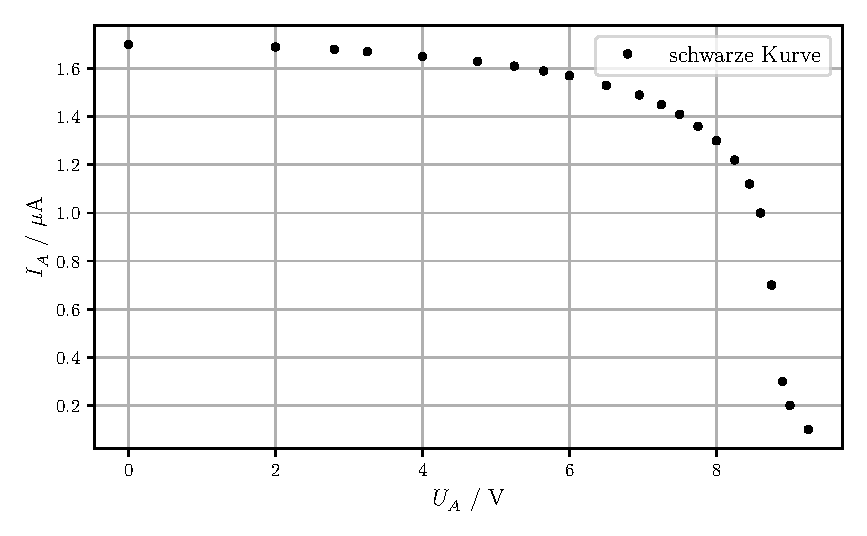
\includegraphics[width=\textwidth]{bilder/integral.pdf}
    \caption{Die integrale Energieverteilung der Elektronen aus den ermittelten Messpaaren.
    Diese entspricht der schwarzen Kurve aus \autoref{fig:originaldaten_teil1}.
    Die Temperatur beträgt hier $\SI{24}{\celsius}$, $U_\text{B}$ ist konstant bei $\SI{10}{\volt}$.}
    \label{fig:integral}
\end{figure}

\begin{figure}
    \centering
    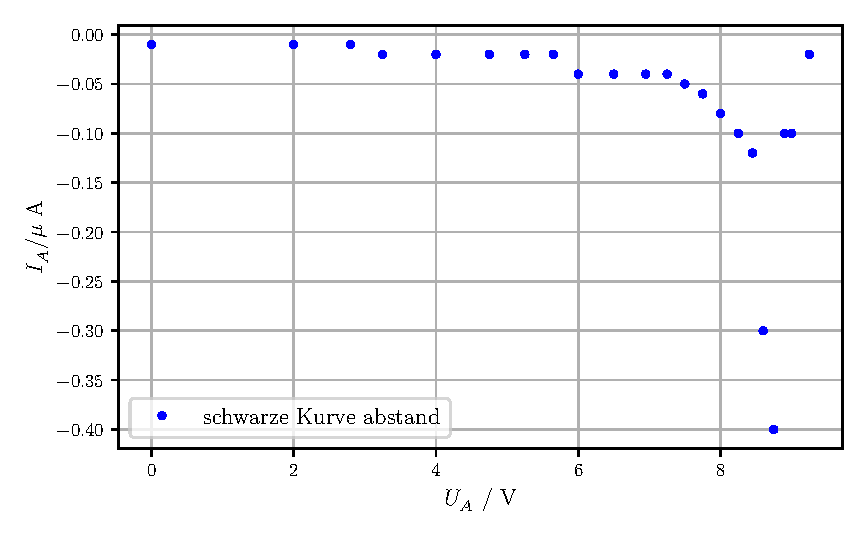
\includegraphics[width=\textwidth]{bilder/abstande.pdf}
    \caption{Die integrale Energieverteilung der Elektronen aus den ermittelten Abständen.
    Hier sind die Abstände $\increment I_\text{A}$ gegen die Bremsspannung $U_\text{A}$ geplottet.}
    \label{fig:abstande}
\end{figure}
\noindent
In \autoref{fig:ableitung} ist die Steigung der integralen Energieverteilung geplottet. \\
Bei $U_\text{A} = \SI{8.75}{\volt}$ kann ein Peak beobachtet werden, dieser ist der Wendepunkt der aufgenommen Energieverteilung.
Das Kontaktpotential kann hierdurch ermittelt werden.
Da die wirkliche Beschleunigungsspannung nicht bei $U_\text{B} = \SI{10}{\volt}$ sondern bei $U_\text{B, eff} = \SI{8.75}{\volt}$ liegt,
folgt nach Gleichung \eqref{eqn:Kontaktpotential} für das Kontaktpotential $K = \SI{1.25}{\volt}$. \\

\begin{figure}
    \centering
    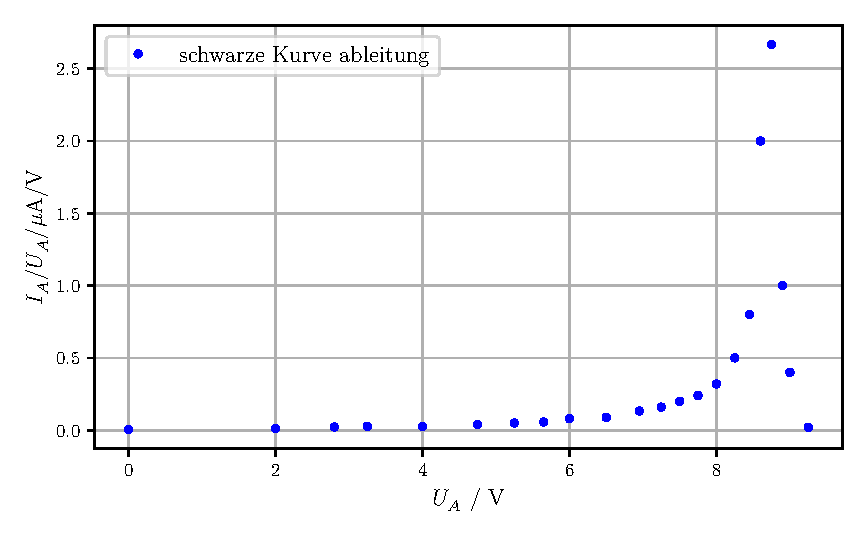
\includegraphics[width=\textwidth]{bilder/ableitung.pdf}
    \caption{Der Betrag der Steigung der integralen Energieverteilung der Elektronen aus den ermittelten Abständen.
    Die rote Linie markiert die Wendestelle, welche die wirkliche Beschleunigungsspannung $U_\text{B, eff}$ markiert.}
    \label{fig:ableitung}
\end{figure}


\noindent
Außerdem wurde eine Kurve bei $T = \SI{145}{\celsius}$ und weiterhin konstanten Beschleunigungsspannung $U_\text{B} = \SI{10}{\volt}$ aufgenommen.
Diese ist in \autoref{fig:originaldaten_teil1} zu sehen. 
Es handelt sich hierbei um die blaue Kurve.
Nach den Gleichung \eqref{eqn:p_sat} und \eqref{eqn:w_bar} kann der Sättigungsdampfdruck $p_\text{sät}$ und die mittlere Weglänge $\bar{w}$ bestimmt werden.
Es folgt
\begin{align*}
    p_\text{sät} &= \SI{3.9804}{\milli\bar} \, , \\
    \bar{w} &= \SI{7.2858e-4}{\centi\metre} \, .
\end{align*}
Somit ist $\bar{w}$ um den Faktor $70000$ größer als $a$.
Die Stoßwahrscheinlichkeit ist dadurch sehr hoch, was an dem Verlauf der Kurve bemerkbar ist.
Die Auffängerstrom $I_\text{A}$ fällt stark ab, was auf viele Stöße deutet.
Dabei kann es sich um viele inelastische aber auch elastische Stöße handeln.
Hier trifft letzteres vermehrt zu, da eine Periodizität der Kurve nicht vorhanden ist.
Zudem ist die Beschleunigungsspannung $U_\text{B}$ zu gering, sodass nur sehr wenige der beschleunigten Elektronen genug Energie haben um mit dem Hg-Atom wirklich wechselwirken zu können.\\
\noindent
Da sich die verwendete Bremsspannung $U_\text{A}$ im selben Intervall befindet, wie in dem Durchlauf zuvor, kann nicht der Hauptgrund für diesen Verlauf des Auffängerstroms sein.
Hier ist das Verhältnis $\sfrac{\bar{w}}{a}$ entscheidend.
Es kommt zu vielen elastischen Stößen zwischen den beschleunigten Elektronen und den Hg-Atomen, was zu Richtungsänderungen führt.
Viele dieser Elektronen kommen also nicht mehr zur Auffängerelektrode.

%%%%%%%%%%%%%%%%%%%%%%%%%%%%%%%%%%%%%%%%%%%%%%%%%%%%%%%%%%%%%%%%%%%%%%%%%%%%%%%%%%%%%%%%%%%%%%%%%%%%%%%%%%%%%%%%%%%%%%%%%%%%%%%%%%%%%%%%%%%%%%%%%%%%%%%%%%%%%%%%%%%%%%%%%%%%%%%%%%%%%%%%%%%
\subsection{Franck-Hertz-Kurve}
Im Folgenden wird die Franck-Hertz-Kurve untersucht.
Die Messung wurde für zwei Temperaturen durchgeführt, zunächst für $T_1 = \SI{200}{\celsius}$ und $T_2 = \SI{176}{\celsius}$.
Die Kurven wurden mit dem XY-Schreiber aufgenommen und sind in \autoref{fig:originaldaten_teil2} zu finden.
Beide Kurven wurden bei einer konstanten Bremsspannung von $U_\text{A}  = \SI{1}{\volt}$ erstellt, dabei ist der Auffängerstrom $I_\text{A}$ gegen die Beschleunigungsspannung $U_\text{B}$ aufgetragen.

\subsubsection{Temparatur $T = \SI{200}{\celsius}$}
Mithilfe der Gleichungen \eqref{eqn:p_sat} und \eqref{eqn:w_bar} kann der Sättigungsdampfdruck $p_\text{sät}$ und somit die mittlere Weglänge $\bar{w}$ berechnet werden.
Es folgt für $T = \SI{200}{\celsius}$
\begin{align*}
    p_\text{sät} &= \SI{26.8551}{\milli\bar} \, , \\
    \bar{w} &= \SI{1.0799e-4}{\centi\metre} \, .
\end{align*}
Da der Abstand $a$ von der Kathode bis zur Auffängerelektrode um den Faktor $10^4$ größer ist, ist eine ausreichende Stoßwahrscheinlichkeit gegeben.\\

\noindent
Zunächst werden die Abstände $\increment U_\text{B}$ der Maxima abgelesen.
Dazu werden die Abstände $\increment x$ in Kästchen abgelesen und mithilfe der Gleichung
\begin{equation}
    \label{eqn:delta_U_B}
    \increment U_\text{B} = \increment x \cdot \frac{\SI{40}{\volt}}{208 \text{Kästchen}}
\end{equation}
berechnet.
Die Ergebnisse sind in \autoref{tab:Abstande_200} zu finden.

\begin{table}
    \centering
    \caption{Die notierten Abstände, sowie die daraus ermittelten Messwerte $\increment U_\text{B}$ bei $T=\SI{200}{\celsius}$.} 
    \label{tab:Abstande_200}
    \begin{tabular}{c S[table-format=1.4]}
    \toprule
    $\increment x /\text{Kästchen}$ & $\increment U_\text{B} / \si{\volt}$\\
    \midrule
      26 &  5.0\\
      24 &  4.6154\\
      26 &  5.0\\
      26 &  5.0\\
      27 &  5.1923\\
      27 &  5.1923\\
      27 &  5.1923\\
    \bottomrule
    \end{tabular}
\end{table}

\noindent
Somit lautet der mittlere Abstand der Maxima
\begin{align*}
    \increment \bar{U}_\text{B} = \SI{5.0275}{\volt} \, .
\end{align*}
\noindent
Daraus folgt mithilfe der Gleichung \eqref{eqn:anregungsenergie} für die Anregungsenergie des Hg-Atoms
\begin{align*}
    E_{01}=\SI{5.0275}{\electronvolt} \, .
\end{align*}
\noindent
Desweiteren kann nach Gleichung \eqref{eqn:lambda} die Wellenlänge $\lambda$ bestimmt werden,
\begin{align*}
    \lambda = \SI{2.4661e-07}{\metre} \, .
\end{align*}

\subsubsection{Temparatur $T = \SI{176}{\celsius}$}
Mithilfe der Gleichungen \eqref{eqn:p_sat} und \eqref{eqn:w_bar} kann der Sättigungsdampfdruck $p_\text{sät}$ und somit die mittlere Weglänge $\bar{w}$ berechnet werden.
Es folgt für $T = \SI{176}{\celsius}$
\begin{align*}
    p_\text{sät} &= \SI{12.3533}{\milli\bar} \, , \\
    \bar{w} &= \SI{2.3475e-4}{\centi\metre} \, .
\end{align*}
Der Abstand $a$ von der Kathode bis zur Auffängerelektrode ist um den Faktor $10^4$ größer, somit ist eine ausreichende Stoßwahrscheinlichkeit gegeben. \\

\noindent
Die Abstände der Maxima $\increment U_\text{B}$ werden notiert, hierzu  werden di Abstände $\increment x$ in Kästchen aufgenommen und mithilfe der Gleichung \eqref{eqn:delta_U_B} berechnet.
Die Ergebnisse sind in \autoref{tab:Abstande_176} aufgenommen.

\begin{table}
    \centering
    \caption{Die notierten Abstände, sowie die daraus ermittelten Messwerte $\increment U_\text{B}$ bei $T=\SI{176}{\celsius}$.} 
    \label{tab:Abstande_176}
    \begin{tabular}{c S[table-format=1.4]}
    \toprule
     $\increment x /\text{Kästchen}$ & $\increment U_\text{B} / \si{\volt}$\\
    \midrule
      26 &  5.0\\
      25 &  4.8077\\
      27 &  5.1923\\
      26 &  5.0\\
      27 &  5.1923\\
      28 &  5.3846\\
    \bottomrule
    \end{tabular}
\end{table}

\noindent
Somit lautet der mittlere Abstand der Maxima
\begin{align*}
    \increment \bar{U}_\text{B} =  \SI{5.0962}{\volt} \, .
\end{align*}
\noindent
Daraus folgt mithilfe der Gleichung \eqref{eqn:anregungsenergie} für die Anregungsenergie des Hg-Atoms
\begin{align*}
    E_{01}=\SI{5.0962}{\electronvolt} \, .
\end{align*}
\noindent
Dadurch kann nach Gleichung \eqref{eqn:lambda} die Wellenlänge $\lambda$ bestimmt werden,
\begin{align*}
    \lambda = \SI{2.4329e-07}{\metre} \, .
\end{align*}